\subsection{Pepper Noise}\label{image_1}
Pepper noise is when a set of pixels on an image are complete black, without the actual photographed scene has these elements.
To find the noise in an image, an uniform area is selected and analysed.
In figure \ref{fig:hist_pepper_im01} can it be seen that the image suffers from pepper noise.
It is assumed that the proportion of pepper in the uniform area is the same as over the whole of the image.

\begin{figure}[H]
\centering

\includegraphics[width = \histogramWidth]{graphics/hist1_uniform.png}
\caption{Histogram of the original ``Image1.png'' showing pepper noise in a uniform area.}
\label{fig:hist_pepper_im01}
\end{figure}

A median filter is good to combat salt and pepper noise as it takes the midpoint and thus avoids extreme values.
This assumes that the amount of salt or pepper is less than 20\% and the filter is large enough to get values which are neither entire salt or entire pepper.
To remove pepper noise from an image with mostly pepper noise, the amount of pepper damage needs to be found.
The image was detected to be 60\% pepper.
This means a median filter is not viable as the midpoint is likely to turn out as pepper.

Knowing this means that the midpoint must be shifted towards a lighter color.
This method is called alpha trimmed mean.
The new midpoint which can be calculated using equation \ref{eq:quantile} and was found to be 80\%. 

\begin{equation}
 q = (\text{pepper}-\text{salt}+1)/2 \label{eq:quantile}
\end{equation}

A 3x3 midpoint filter is applied to the image to remove the majority of the damage to the image.
Then a 7x7 alpha trimmed mean with a width of 3 is applied to further remove the pepper noise.
Running a median filter twice gives the effect of overestimating the damage of the pepper and thus results in a brighter image.

To see if the filters does damage to the original image an area with more complex features are shown.
In figure \ref{fig:complex1_after_alpha} can the area be seen after the alpha trimmed mean filter has been applied.
It can be seen that there is still noise present in the image.

\begin{figure}[H]
\centering
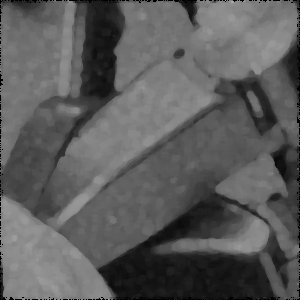
\includegraphics[width = \cutOutWidth]{graphics/complex1_step2}
\caption{Image in a complex area after alpha trimmed mean filter.}
\label{fig:complex1_after_alpha}
\end{figure}

To see the noise, another histogram of the uniform area is made.
In figure \ref{fig:hist_img1_after_alpha} can the histogram of the uniformed area after the applying two filters be seen.
The histogram suggest that there is still Gaussian noise in the image.
Gaussian noise can be removed by applying an arithmetic mean filter.

\begin{figure}[H]
\centering
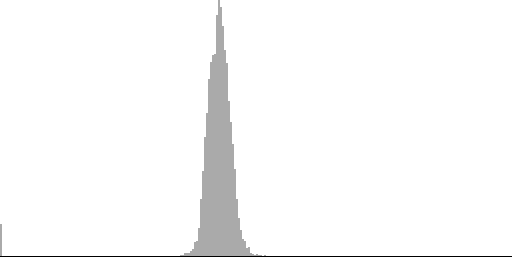
\includegraphics[width = \histogramWidth]{graphics/hist1_uniform2.png}
\caption{Histogram of the filtered uniform area after alpha trimmed mean filter.}
\label{fig:hist_img1_after_alpha}
\end{figure}

In figure \ref{fig:complex1_after_blur} can the effect of applying arithmetic mean to the image be seen.
By taking the image into logarithmic space, the noise becomes additive and thus can be separated with a arithmetic mean filter.
In figure \ref{fig:complex1_after_harmonic} can the effect of using a harmonic mean arithmetic mean filter be seen.
Both filters have the size of 5x5. The Difference is not that obvious from visual inspection so the difference is calculated using equation \ref{eq:img_diff_harVSgeo}.

\begin{equation}
I_{diff} = \left( I_{har} - I_{geo} \right) * A + 127
\label{eq:img_diff_harVSgeo}
\end{equation}

The difference is shown in figure \ref{fig:complex1_blur_difference}.
The difference is amplified 50 times in order to get a clear contrast between the two.
Darker areas means regular blurring contains higher values.
The most distinct difference between the images is the edges. 
The edges are brighter after the regular filter. 
The most visible edges on the difference image occurs where the image goes from a large area of light to a small area of dark.
Thus the edges are better preserved on the harmonic mean filter.
In the lower right corner, the underside of the gripper is supposed to be dark.
Therefore having higher values with the regular filter gives unwanted bright spots which the harmonic mean filter removes.
It is therefore concluded that the harmonic mean filter is the best for this task.



\begin{figure}[H]
\centering
  \begin{subfigure}{\linewidth}
  \centering
    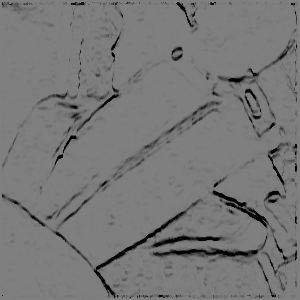
\includegraphics[width = \cutOutWidth]{graphics/complex1_blurr_difference_50.png}
    \caption{Difference.}
    \label{fig:complex1_blur_difference}
  \end{subfigure}
  
  \begin{subfigure}{\cutOutWidth}
    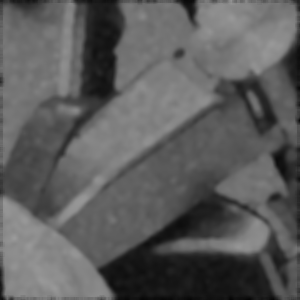
\includegraphics[width = \textwidth]{graphics/complex1_blurred.png}
    \caption{Geometric Mean.}
    \label{fig:complex1_after_blur}
  \end{subfigure}
%
  \begin{subfigure}{\cutOutWidth}
    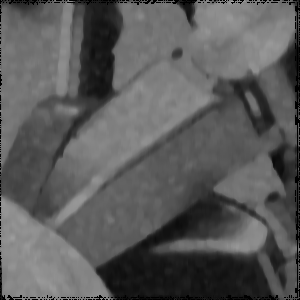
\includegraphics[width = \textwidth]{graphics/complex1_harmonic_blurred.png}
    \caption{Harmonic mean.}
    \label{fig:complex1_after_harmonic}
  \end{subfigure}
\caption{Image in a complex area after applying different mean filters.}
\end{figure}

The resulting sequence is thus:
\begin{itemize}
 \item Shifted midpoint filter, kernel size 3x3, quantile of 80\%.
 \item Alpha mean filter, kernel size 7x7, quantile of 80\%, mean width of 3.
 \item Harmonic mean filter, kernel size 5x5.
\end{itemize}

The final image of image 1 can be seen in figure \ref{fig:final_image1}.

\begin{figure}[H]
\centering
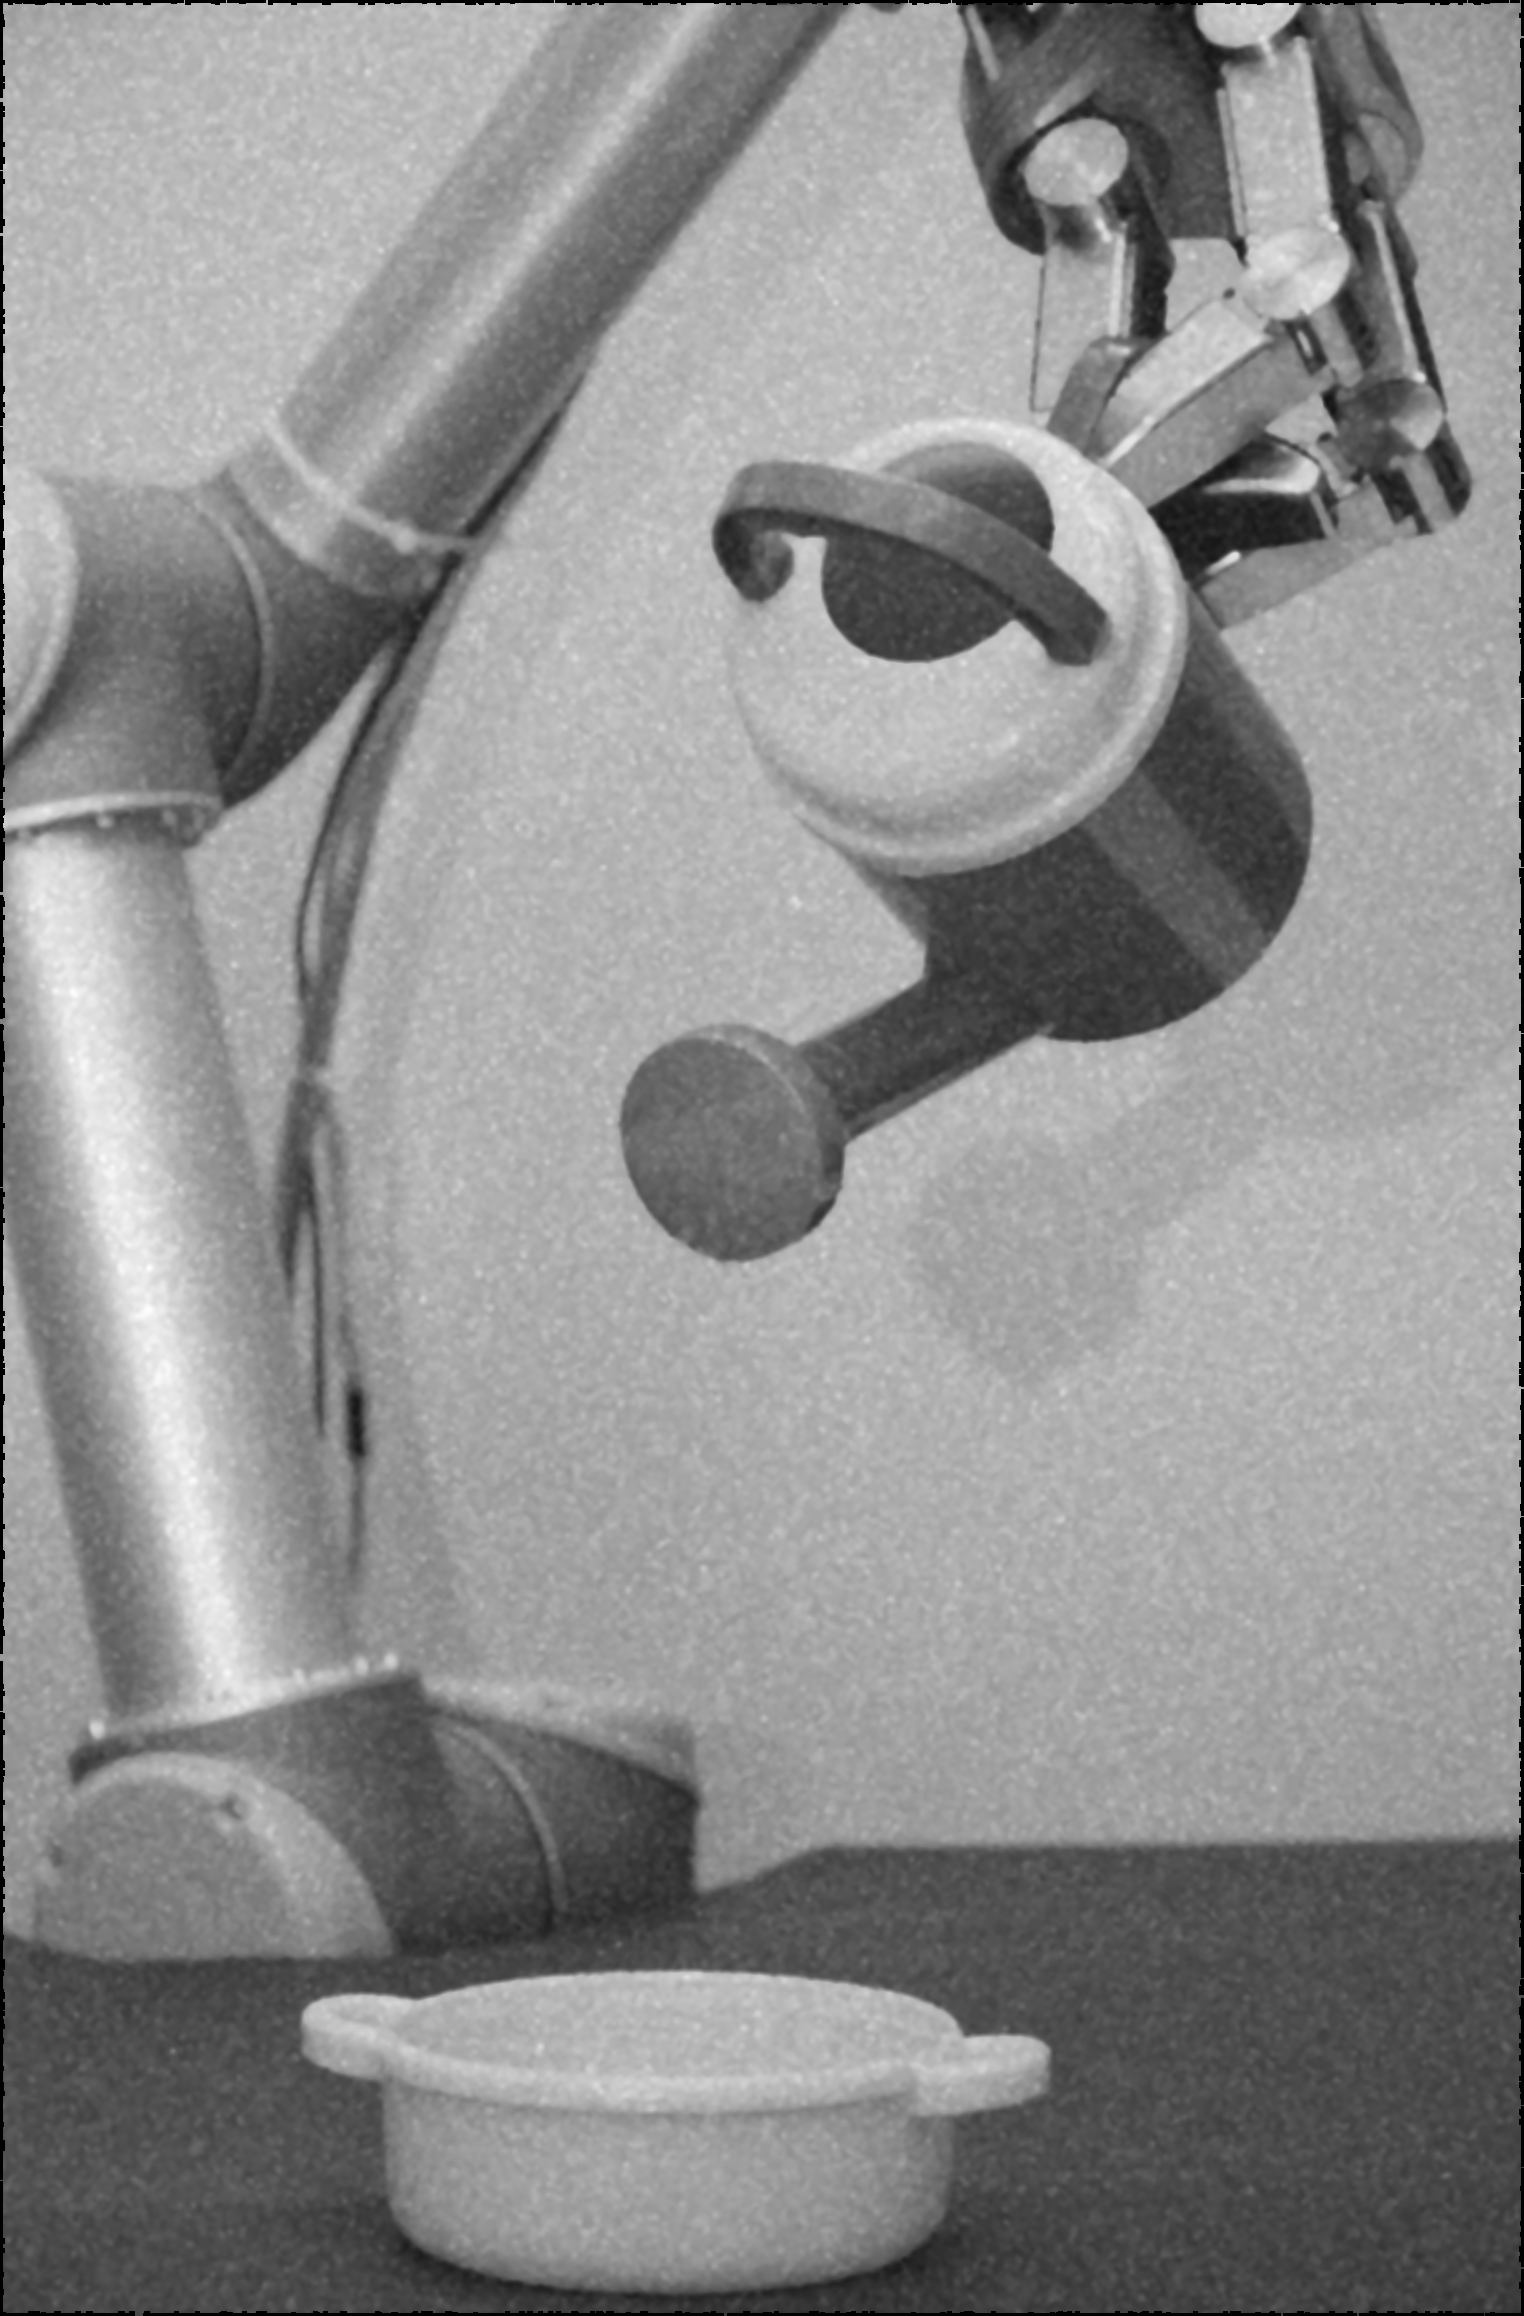
\includegraphics[width = \fullImageWidth]{../code/images/image_result_1.png}
\caption{Image 1 restored.}
\label{fig:final_image1}
\end{figure}
